%% ID: phil_masses_pivot
%% TITLE: Bismar Scales
%% TYPE: question
%% QUESTIONTYPE:  numerical
%% CONCEPTS: forces, moments, newtoni
%% VIDEOS: 
%% LEVEL: 3
%% TOPIC: mechanics/statics
%% ORDER: 7


\begin{problem}[Phil_masses_pivot]
{\exposition{Bismar scales are a type of scale used to weigh merchandise cheaply and quickly without the need for many weights. The scales consist of a light rod with a known mass attached to one end. The mass to be weighed is then attached to the other end and the pivot point is moved until the scales are in equilibrium.}

\nl \question{A particular Bismar scale is made up of a light rod AB with length \value{l}{50}{cm} and a fixed mass \value{m_1}{0.7}{kg} at A. A second mass \vari{m_2} is suspended from B. If the rod is in equilibrium when the pivot point is \quantity{16}{cm} from A, find \vari{m_2}. Give your answer to 2 significant figures.}
}
{\textit{Created for the Rutherford School Physics Project by PS.}}
{\answer{\valuedef{m_2}{0.33}{kg}}
\begin{figure} [h]
	\centering
	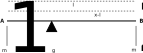
\includegraphics[width=0.4\textwidth]{../../../figures/Statics_masses_pivot.svg}
	\caption{}
	\label{fig:Statics_masses_pivot}
\end{figure}
If the rod is in equilibrium then there must be no resultant moment acting about the pivot. On the diagram in Figure \ref{fig:Statics_masses_pivot} the distance from A to the pivot has been marked as \vari{x}. Taking moments about the pivot:
\begin{equation*}	
m_1gx = m_2g\left(l - x\right)	
\end{equation*}
\begin{equation*}	
\Rightarrow m_2 = \frac{m_1x}{l-x}	
\end{equation*}
Substituting in \value{m_1}{0.7}{kg}, \value{x}{0.16}{m} and \value{l}{0.5}{m}:
\begin{equation*}	
m_2 = \frac{0.7 \times 0.16}{0.5 - 0.16} = 0.33 \textrm{ kg}	
\end{equation*}
}
\end{problem}